\documentclass[conference]{IEEEtran}
\IEEEoverridecommandlockouts
% The preceding line is only needed to identify funding in the first footnote. If that is unneeded, please comment it out.
\usepackage{cite}
\usepackage{amsmath,amssymb,amsfonts}
\usepackage{algorithmic}
\usepackage{graphicx}
\usepackage{textcomp}
\usepackage{natbib}
\usepackage{float}
\usepackage{xcolor}
\bibliographystyle{plainnat}
\def\BibTeX{{\rm B\kern-.05em{\sc i\kern-.025em b}\kern-.08em
    T\kern-.1667em\lower.7ex\hbox{E}\kern-.125emX}}
\begin{document}

\title{Machine Learning Approaches for Accurate Diamond Price Prediction\\
% {\footnotesize ECS-171 Final Project: \textbf{Group 21}}
\thanks{Final Project Report ECS-171: \textbf{Group 21}}
}

\author{
\IEEEauthorblockN{Aditya Mittal}
\IEEEauthorblockA{\textit{Department of Statistics} \\
\textit{University of California, Davis}\\
Davis, United States \\
adimittal@ucdavis.edu}
\and
\IEEEauthorblockN{Andrew Yeow}
\IEEEauthorblockA{\textit{Department of Computer Science} \\
\textit{University of California, Davis}\\
Davis, United States \\
XXX}
\and
\IEEEauthorblockN{Yifan Cui}
\IEEEauthorblockA{\textit{Department of Computer Science} \\
\textit{University of California, Davis}\\
Davis, United States \\
XXX}
\and
\IEEEauthorblockN{Nandini Koladi}
\IEEEauthorblockA{\textit{Department of Computer Science} \\
\textit{University of California, Davis}\\
Davis, United States \\
XXX}
\and
\IEEEauthorblockN{Eshan Toshniwal}
\IEEEauthorblockA{\textit{Department of Computer Science} \\
\textit{University of California, Davis}\\
Davis, United States \\
XXX}
}

\maketitle

\begin{abstract}
In 2023, the U.S. jewelry market was valued at 73.32 billion USD, with diamonds comprising a significant share. Predicting diamond prices accurately is essential for jewelers to make informed pricing decisions. This paper explores various machine learning algorithms, including linear regression, Random Forests, XGBoost, and neural networks, to predict diamond prices based on characteristics such as carat, cut, color, and clarity. Through exploratory data analysis, we identify key features influencing diamond prices and apply these insights to improve model performance. Our methodology includes rigorous model evaluation using metrics like Mean Squared Error (MSE), Mean Absolute Error (MAE), and R-squared (R²). By developing a robust predictive model, we aim to enhance pricing precision, benefiting both businesses and consumers in the diamond market.
\end{abstract}

\begin{IEEEkeywords}
Diamond pricing, machine learning, predictive modeling, neural network, decision trees
\end{IEEEkeywords}

\section{Introduction}

In 2023, the jewelry market in the United States was estimated to be worth 73.32 billion USD, with projections for 2024 reaching 96.61 billion USD \cite{us}. Clearly, the market for jewelry is quite significant and continues to display steady growth. In particular, \emph{diamonds} account for a significant portion of this market, covering an estimated 50-60\% market share as compared to some of the other precious stones such as gold, silver, etc \cite{diamond}. Consequently, it becomes important for jewelers to adopt accurate methods to predict prices of these diamonds to better serve their consumers. In fact, businesses have began educating their sellers on essential qualities such as cut, color, carat weight, and clarity to make informed pricing decisions. As such, ensuring accurate price predictions becomes very important as it has significant financial implications on both businesses and consumers alike.

Given the importance of this task, it becomes crucial to develop methods that enable accurate prediction of prices for these diamonds. Machine learning, with its ability to learn patterns in data and generate predictions, has become extremely popular in recent years across a wide range of applications \cite{kino}. Recent advancements in machine learning have introduced a range of algorithms, including linear regression, K-Nearest Neighbors, Random Forests, and the increasingly popular neural networks \cite{sarker}. In this paper, we explore several different machine learning algorithms to accurately predict diamond prices based on their given characteristics, including those mentioned above. The application of creating models to generate accurate predictions is widespread, as it can aid jewelers and marketers who aim to provide accurate pricing methods for consumers in the jewelry market.

Our dataset contains several essential features for diamond price prediction, such as the aforementioned carat, cut, color, clarity, etc. \cite{kaggle} Through exploratory data analysis (EDA), we aim to understand how these features are related to diamond pricing. This analysis will help us answer questions about which features most significantly impact diamond prices and ways we can leverage this information to create accurate predictive models. Ultimately, our goal is to develop an accurate model for predicting diamond prices, enabling jewelers to make precise pricing decisions and improving the overall consumer purchasing experience. This paper details our methodology, including EDA and the application of various machine learning algorithms, to achieve this objective.

The outline of this paper is as follows: Section 2 reviews the related literature on diamond price prediction and provides a historical perspective on machine learning and relevant algorithms. Section 3 presents data description and exploratory data analysis. Sections 4 and 5 highlight the proposed methodology and results. Finally, the paper concludes with a discussion and future perspective in Section 6.

\section{Literature Review}

Much literature has been published to develop predictive models for accurately estimating diamond prices, using various social contexts and individual diamond characteristics. Alsuraihi et al. \cite{Alsuraihi} aimed to develop an accurate algorithm to estimate diamond prices. They considered various features such as diamond sizes and other key factors. Various machine learning methods were tested, including Linear Regression, Random Forest Regression, Polynomial Regression, Gradient Descent, and Neural Networks. Similarly, Mamonov and Triantoro \cite{Mamonov} studied the relationship between a diamond's physical attributes and respective prices in e-commerce contexts, with the goal of understanding how these attributes affect diamond prices. However, their study did not account for the diamond cut, a significant factor affecting market value, which is included in our dataset. Pandey et al. \cite{Pandey} addressed the challenge of forecasting future values of precious metals like gold and diamonds. They used ensemble approaches combined with feature selection techniques to enhance prediction accuracy. In an alternate perspective, Scott and Yelowitz \cite{Scott} investigated diamond prices in the context its social status and intrinsic value. They collected data from online diamond sellers and empirically examined factors influencing diamond prices, considering carat weight, color, cut, and clarity in determining the logarithm of price. Clearly, a variety of approaches have been taken to create accurate prediction models, ranging from investigating social contexts to individual characteristics. In this paper, we utilize several algorithms to create accurate models ourselves. The latter half of this section provides an overview of key machine learning algorithms of this paper, including regression models, decision trees, and artificial neural networks. We examine the Grid Search method for hyperparameter tuning.

\subsection{Linear Regression}

Linear regression is one of the simplest and most interpretable prediction models. It fits a straight line between the response variable $Y$ and predictors $X$. The goal of this model is to minimize the Residual Sum of Squares (RSS) \cite{Seber}:

\[
\text{RSS} = \sum_{i=1}^n (y_i - \hat{y}_i)^2
\]

Linear regression assumes linearity, independence, homoscedasticity, and normality of residuals \cite{Kutner}. It is evaluated using metrics like $R^2$ and Mean Squared Error (MSE). Extensions include multiple linear regression, polynomial regression, and regularization methods like Ridge and Lasso regression to handle complex relationships and prevent overfitting \cite{Wright, Weisberg}.

\subsection{Decision Trees}

Decision trees are very effective on tabular data, as it displays strong performance on both regression and classification tasks. These models split the data based on feature values, forming a tree-like structure. In particular, decision trees are prone to overfitting. Ensemble methods, such as Random Forests \cite{Breiman} and Gradient Boosting Machines like XGBoost \cite{Chen}, mitigate this issue by combining multiple trees, thereby enhancing performance and robustness.

\subsection{Neural Networks}

Neural networks have recently become extremely popular with advances in deep learning and computation ability to handle big data problems \cite{LeCun}. These models consist of layers of interconnected nodes (neurons) that learn representations from data. Rumelhart et. al \cite{Rumelhart} introduced the backpropagation algorithm in order to learn the model weights by minimizing the training loss. Modern neural networks use optimizers like Adam (Adaptive Moment Estimation), which combines adaptive learning rates and momentum for efficient training.

\subsection{Grid Search}

Both Neural Networks and decision trees include a variety of hyperparameters that significantly impact their performance and overall generalization ability on unseen data. Grid search is a method for hyperparameter tuning that evaluates a predefined set (grid) of hyperparameters and finds the optimal configuration among them. This method is quite computationally heavy, as it explore every configuration among the given hyperparameter space to identify the most suitable combination for a given problem. Bergstra and Bengio (2012) \cite{Bergstra} discussed grid search's efficiency and limitations, highlighting its importance in fine-tuning machine learning models for optimal performance.

Therefore, our literature review provides an overview of the research conducted on predicting diamond prices, including discussions on pertinent algorithms such as linear regression, decision trees, and neural networks. For hyperparameter tuning, we plan to utilize Grid Search to optimize the performance of both the decision trees and neural network models.

\section{Dataset Description and Exploratory Data Analysis}

The \emph{diamond prices} dataset contains detailed information about 54,000 diamonds, including their prices and various characteristics \cite{kaggle}. The predictor variables in this dataset are as follows: i) \textbf{Carat}: Represents the weight of the diamond, ranging from 0.2 to 5.01 carats. ii) \textbf{Cut Quality}: Categorized as Fair, Good, Very Good, Premium, or Ideal, indicating the craftsmanship involved in shaping the diamond. iii) \textbf{Color}: Graded from J (worst) to D (best), reflecting the hue and saturation of the stone. iv) \textbf{Clarity}: Measures how clear the diamond is, with grades ranging from I1 (worst), SI2, SI1, VS2, VS1, VVS2, VVS1, to IF (best). v) \textbf{Dimensions}: Captured by the length (x), width (y), and depth (z) in millimeters, with ranges of 0–10.74 mm, 0–58.9 mm, and 0–31.8 mm, respectively. vi) \textbf{Depth Percentage}: Ranges from 43\% to 79\%. vii) \textbf{Table}: Represents the width of the top of the diamond relative to its widest point, ranging from 43\% to 95\%. The dataset does not contain any missing values, so we do not need to any address missing data in the exploratory data analysis step.

\subsection{Exploratory Data Analysis}

To explore the dataset further and understand the relationships between these features and diamond prices, we will conduct exploratory data analysis (EDA). First, we visualize the distribution of each continuous feature, such as carat, length (x), width (y), depth (z), depth percentage, and table, to understand their spread and central tendencies. A table will highlight the mean, median, and standard deviation statistics of each feature, providing insights into their individual magnitudes and spread. Second, pairwise scatter plots display the relationship between each continuous feature and diamond price, helping to identify potential trends and correlations. Third, the correlation heat-map presents Pearson correlation relationships between continuous features, helping identify features most correlated with price. Finally, we create histograms of categorical features like cut, color, and clarity to understand their distributions. These visualizations provide insights into the structure of the data, highlight any anomalies, and help with subsequent modeling efforts to predict diamond prices effectively.

\begin{figure}[H]
    \centering
    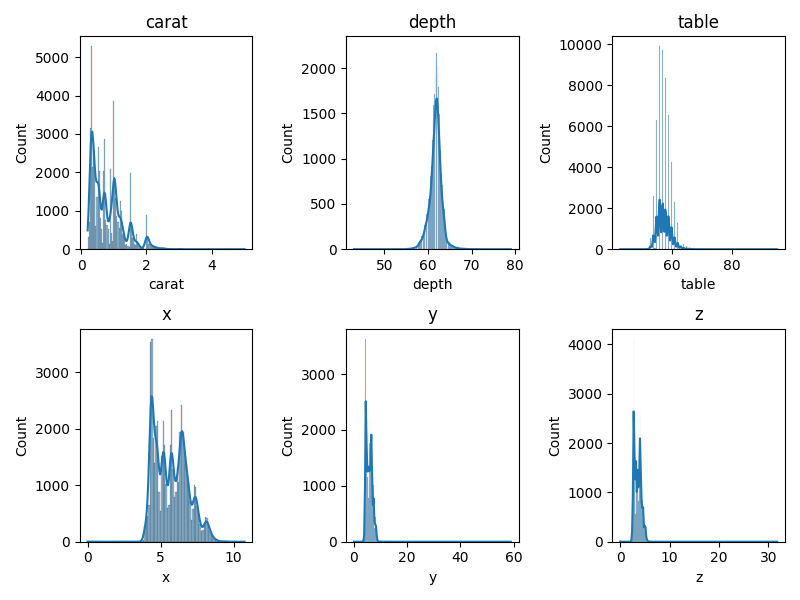
\includegraphics[width=0.8\linewidth]{Figure_1.png}
    \caption{Distribution Plot of Continuous Features. Identify trends our dataset such as skewness, location of outliers, mean, median, scale, etc.}
    \label{fig:image_label}
\end{figure}

The distribution of continuous predictors highlight potential skewness in our dataset. For instance, the predictor \emph{carat} suggests potential skewness to the right – with many upper outliers – as evidenced by its distribution plot. This trend holds true for features \emph{y} and \emph{z} as well. These plots suggest that our dataset may contain a significant number of upper outliers, which we will consider removing in the data pre-processing stage. To further gain insight on the distribution of our continuous features, the table below summarizes the mean, median, and standard deviation of the each predictor:

\begin{table}[H]
    \centering
    \caption{Mean, Median, Standard Dev. of Continuous Features}
    \label{tab:example_table}
    \begin{tabular}{|c|c|c|c|}
        \hline
        Feature & Mean & Median & Standard Dev. \\
        \hline
        Carat & 0.797 & 0.70 & 0.474 \\
        \hline
        Depth & 61.749 & 61.80  & 1.432 \\
        \hline
        Table & 57.457 & 57.00 & 2.234 \\
        \hline
        X & 5.731 & 5.70 & 1.122 \\
        \hline
        Y & 5.734 & 5.71 & 1.142 \\
        \hline
        Z & 3.538 & 3.53 & 0.705 \\
        \hline
    \end{tabular}
\end{table}

From our table, we can observe that the mean and median values for most features are relatively close, indicating that the data distributions may not actually be as heavily skewed for most variables. However, the standard deviation values highlight the variability within each feature, such as carat and dimensions (x, y, z), display considerable spread. This variability and potential skewness (from the plots), especially in the carat feature from the plots, could influence our predictive algorithms. Next, we will create pairwise scatter-plots to identify trends between diamond prices and the features.

\begin{figure}[H]
    \centering
    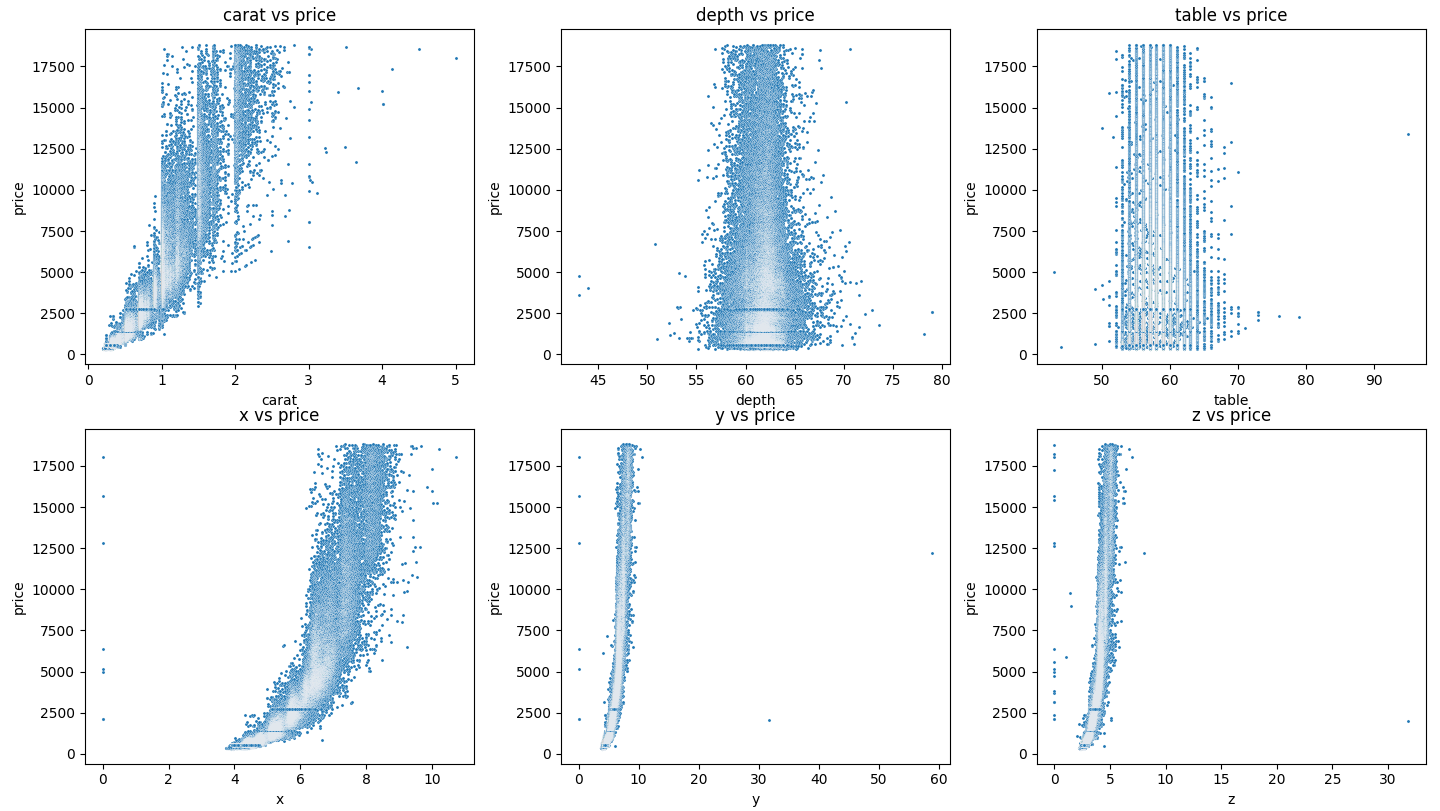
\includegraphics[width=0.8\linewidth]{Figure_4.png} % Replace "example-image" with the filename of your image
    \caption{Pair-wise Scatterplots for Each Feature vs. Diamond Price}
    \label{fig:image_label}
\end{figure}

From the scatterplots of each feature against the response variable, we observe a quadratic relationship between the features, carat, x, y, and z, with respect to the the response variable price. This suggests that a polynomial regression model might be suitable for our dataset in addition to a linear regression model. Thus, we will evaluate the polynomial regression model's performance on the dataset compared to traditional linear regression. Next, we will also analyze the correlations between these continuous features and the target variable, price, to determine the most influential predictors. This will allow us to identify the most relevant features and also potential multicollinearity and interactions.

\begin{figure}[H]
    \centering
    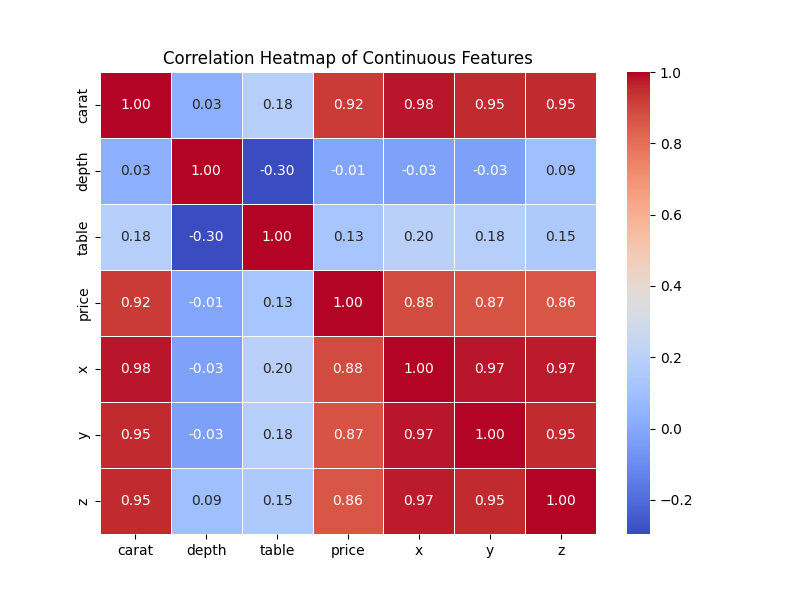
\includegraphics[width=0.8\linewidth]{Figure_3.png} % Replace "example-image" with the filename of your image
    \caption{Correlation Heat-Map for Continous Features vs Diamond Price}
    \label{fig:image_label}
\end{figure}

Based on the results of our correlation heatmap, the feature \emph{Carat} appears to be highly correlated with price, with a correlation coefficient of 0.92. Similarly, it is correlated with dimension features \emph{x}, \emph{y}, and \emph{z}. This makes sense, as carat weight would directly relate to diamond size. Thus, this plot suggests that Carat (and potentially dimensions) are the strongest predictors for diamond price. We showcase data preprocessing methods for outlier removal using carat below. On the other hand, both depth percentage and table have almost zero correlation, indicating that they do not have much association with diamond prices. Thus, this heatmap is insightful in identifying the key predictors for diamond prices and guiding our feature selection process. Next, we will examine histograms for the distribution of categorical features cut, clarity, and color:

\begin{figure}[H]
    \centering
    \includegraphics[width=0.8\linewidth]{figure_5.png} % Replace "example-image" with the filename of your image
    \caption{Historgram for the distribution of categorical features: Cut, Clarity, and Color }
    \label{fig:image_label}
\end{figure}

The histogram of the categorical variables displays their frequencies. Upon initial analysis of the plot, we observe that the cut category "Ideal" appears most frequently, followed by "Premium" and "Very Good," while the "Fair" cut appears least frequently. The distribution of color appears to be well spread, with all colors represented. Regarding clarity, categories such as "I1" and "IF" have relatively few observations compared to others. With this, our exploratory data analysis step has provided valuable insights into the structure of the dataset and identify patterns among the features. We will now proceed with data pre-processing before implementing our machine learning algorithms.

\subsection{Data Pre-Processing} 

Before implementing the machine learning algorithms, we conducted several pre-processing steps on our dataset. First, considering the ordinality present in each of our categorical features, we implemented label encoding to convert these features into numeric representations. The mappings for each categorical feature were defined as follows:

\begin{table}[htbp]
    \centering
    \caption{Label Encodings for Categorical Features}
    \resizebox{\columnwidth}{!}{
        \begin{tabular}{|l|l|}
            \hline
            \textbf{Feature} & \textbf{Encoding} \\
            \hline
            Cut & 'Fair': 0, 'Good': 1, 'Very Good': 2, 'Premium': 3, 'Ideal': 4 \\
            Color & 'J': 0, 'I': 1, 'H': 2, 'G': 3, 'F': 4, 'E': 5, 'D': 6 \\
            Clarity & 'I1': 0, 'SI2': 1, 'SI1': 2, 'VS2': 3, 'VS1': 4, 'VVS2': 5, 'VVS1': 6, 'IF': 7 \\
            \hline
        \end{tabular}
    }
    \label{tab:label_encodings}
\end{table}

Next, to standardize our data and balance the scale of our features, we applied z-score transformation. This transformation ensures that all our features have a mean of 0 and a standard deviation of 1, thereby balancing the scales among features. This is particularly beneficial for algorithms such as neural networks. Finally, we proceeded to remove outliers. Since carat was our most highly correlated predictor, we used it as the feature to identify and remove outliers using the 1.5 times the interquartile range (IQR) calculation. Approximately 3.9\% of the dataset was removed through this process, leaving us with 51,800 rows of data. The boxplots for each feature post outlier removal are shown below:

\begin{figure}[H]
    \centering
    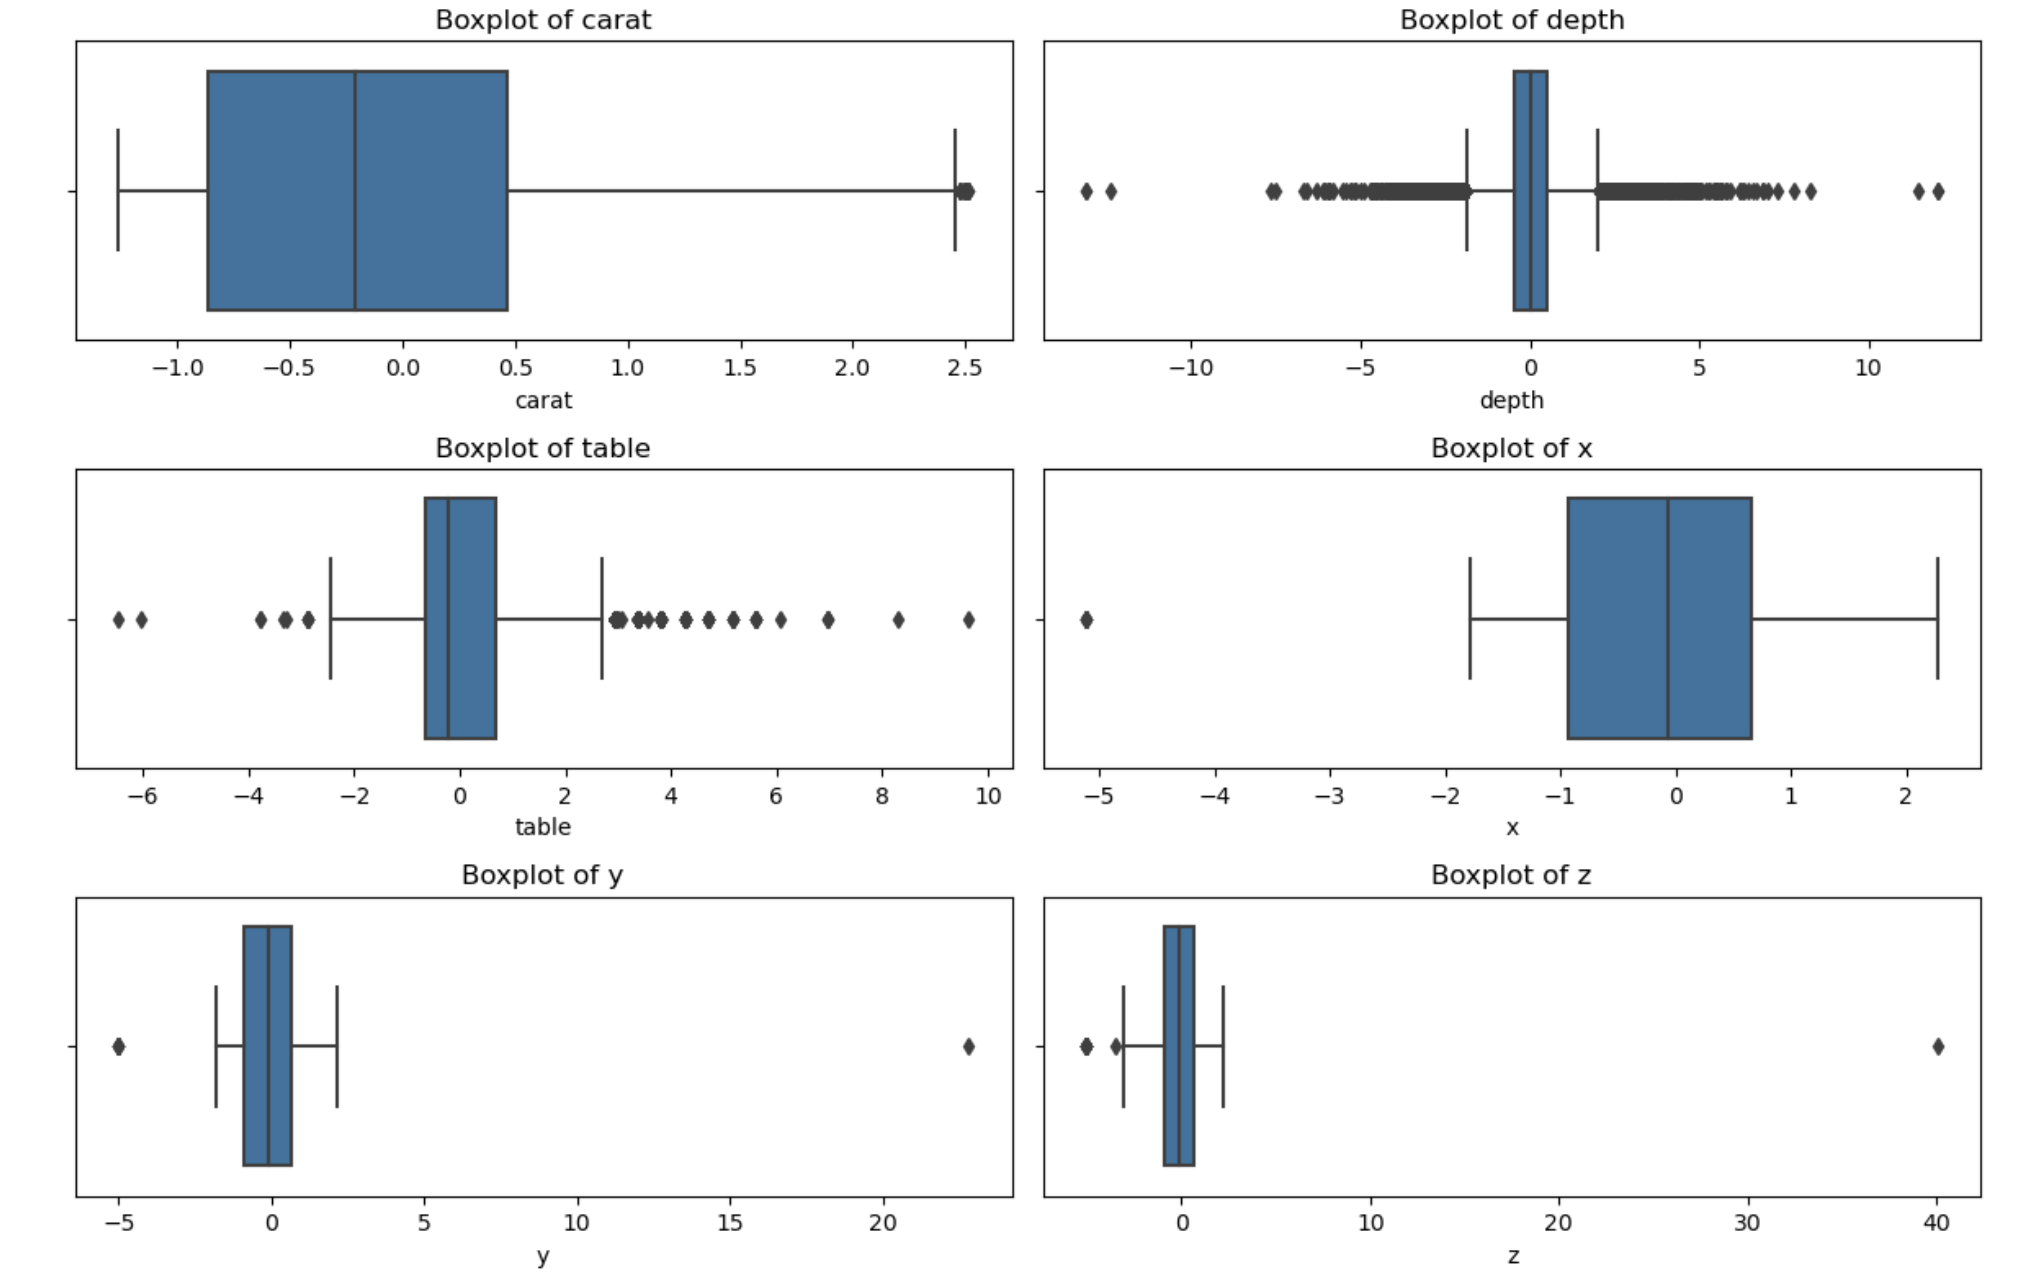
\includegraphics[width=0.8\linewidth]{boxplot.png} % Replace "example-image" with the filename of your image
    \caption{Boxplots of Features Post-Outlier Removal}
    \label{fig:boxplots}
\end{figure}

The boxplots indicate that outliers were removed for carat, while several other features such as depth and table still exhibit upper values. Since these features are not highly correlated with our response variable, we decided to keep them as is and proceed with this cleaned version of the dataset. 

\section{Proposed methodology}

In this paper, we will explore the predictive capabilities of several machine learning algorithms, ranging from linear regression, decision trees, and artificial neural networks. Our approach involved several steps to develop and evaluate model performance to choose the most accurate algorithm. Data preprocessing has already been completed as described above.

\subsection{Linear Regression}

We begin with linear regression model to fit a straight-line model between diamond prices and the aforementioned features. This initial step helps us gain intuition about the relationship between the features and diamond prices using a simple model. From our EDA step, since price displayed a quadratic relationship with carat and diamond dimensions (x,y,z), we also test the performance of a polynomial regression model by including squared terms of these respective features. Thus, we can capture potential nonlinear relationships and assess whether polynomial regression outperforms traditional linear regression.

\subsection{Decision Trees} 

For decision tree-based models, we employ two algorithms; Random Forests and XGBoost. Random Forests aggregate the predictions of multiple decision trees to enhance accuracy and reduce overfitting; XGBoost is a gradient boosting algorithm that iteratively optimizes the model to minimize overall error. We implement grid search with a 5-fold cross-validation to identify the optimal set of hyperparameters. These are the following set of hyper-parameters we tested: 

\begin{itemize}
    \item \textbf{Random Forests}: Our parameter grid explores options for 'bootstrap' (set to True), 'max\_features' ('auto' and 'sqrt'), 'max\_depth' (None, 10, and 20), 'min\_samples\_leaf' (1 and 2), 'min\_samples\_split' (2 and 5), and 'n\_estimators' (100, 200, and 300).
    \item \textbf{XGBoost}: We examine hyperparameters such as 'max\_depth' (3, 6, and 9), 'learning\_rate' (0.1 and 0.01), 'n\_estimators' (100, 200, and 300), 'subsample' (0.8 and 1.0), 'colsample\_bytree' (0.8 and 1.0), 'gamma' (0 and 0.1), 'reg\_alpha' (0 and 0.1), and 'reg\_lambda' (0 and 0.1).
\end{itemize}

This broad range of values for each hyperparameter enables us to explore a wide array of model configurations and identify the optimal combination for our dataset. Subsequently, we train the model using this set of hyperparameters on the training data and assess its performance on the testing set. The plot of training and testing loss vs.\ epoch is provided to demonstrate model performance.

\subsection{Artificial Neural Networks}

In our exploration of predicting diamond prices, we employ artificial neural networks (ANNs). Our ANN architecture consists of a single hidden layer with ReLU activation, followed by an output layer also utilizing ReLU activation, as our task involves regression. To optimize the performance of our ANN, we conduct a grid search for hyperparameter tuning, aiming to select the most suitable parameters for our model. We explore the following hyperparameters during grid search with a 5-fold cross-validation procedure. We explore the following set of hyperparameters:

\begin{itemize}
    \item 'learning\_rate' (0.001, 0.0001)
    \item 'momentum' (0.5, 0.9)
    \item 'number of neurons in hidden layer' (16, 32, 64)
    \item 'dropout\_rate' (None, 0.2, 0.3)
    \item 'batch\_size' (256, 512, 1028)
\end{itemize}

By evaluating these hyperparameters, we will to identify the optimal configuration of hyperparameters that maximizes the predictive performance of our ANN model on the given dataset. Additionally, we incorporate the Adam optimizer into our ANN model to further improve the training process and overall predictive accuracy.


\subsection{Evaluating Model Performance}

In our grid search, we will use the \emph{negative mean squared error} as our metric to identify the optimal set of hyperparameters for both decision trees and the artificial neural network. To assess the performance of our models on the testing data, we will compare their results using several metrics, including Mean Squared Error (MSE), Mean Absolute Error (MAE), and R-squared ($R^2$) between the true values and our predictions. These metrics will help evaluating the accuracy and fit of each algorithm on the testing data. By analyzing these measures, our goal is to find the most effective algorithm for predicting diamond prices as it offers valuable insights for jewelers and marketers in the industry. Through this methodology, we will develop an accurate for predicting diamond prices, leveraging the strengths of various machine learning techniques and achieve best performance possible.

\section{Experimental results and evaluation}

Our experimental methodology provides nuanced results across each of the machine learning algorithms. In particular, the results are as follows:

\subsection{Linear \& Polynomial Regression}

In terms of our training data, we tested the effectivness of both linear and polynomial regression models on our training data using 5-Fold Cross validation. Based on the results, this was our mean score error on training data:

\begin{table}[h]
\centering
\begin{tabular}{|c|c|c|}
\hline
Column 1 & Column 2 & Column 3 \\
\hline
Row 1 & Cell 1 & Cell 2 \\
Row 2 & Cell 3 & Cell 4 \\
Row 3 & Cell 5 & Cell 6 \\
Row 4 & Cell 7 & Cell 8 \\
\hline
\end{tabular}
\caption{A simple table with 3 columns and 4 rows.}
\label{tab:mytable}
\end{table}


\subsection{Decision Trees}

\textbf{Random Forest Algorthm}

For our decision tree algorirhtms, the results of grid searhc provided the following best set of hyperpatemrs for our random forest algorhtm.

\begin{table}[h]
\centering
\begin{tabular}{|c|c|c|}
\hline
Column 1 & Column 2 & Column 3 \\
\hline
Row 1 & Cell 1 & Cell 2 \\
Row 2 & Cell 3 & Cell 4 \\
Row 3 & Cell 5 & Cell 6 \\
Row 4 & Cell 7 & Cell 8 \\
\hline
\end{tabular}
\caption{A simple table with 3 columns and 4 rows.}
\label{tab:mytable}
\end{table}

\textbf{XGBoost} 

\begin{table}[h]
\centering
\begin{tabular}{|c|c|c|}
\hline
Column 1 & Column 2 & Column 3 \\
\hline
Row 1 & Cell 1 & Cell 2 \\
Row 2 & Cell 3 & Cell 4 \\
Row 3 & Cell 5 & Cell 6 \\
Row 4 & Cell 7 & Cell 8 \\
\hline
\end{tabular}
\caption{A simple table with 3 columns and 4 rows.}
\label{tab:mytable}
\end{table}

\subsection{Neural Network}

The grid search for neural network presents the following results: 

\begin{table}[h]
\centering
\begin{tabular}{|c|c|c|}
\hline
Column 1 & Column 2 & Column 3 \\
\hline
Row 1 & Cell 1 & Cell 2 \\
Row 2 & Cell 3 & Cell 4 \\
Row 3 & Cell 5 & Cell 6 \\
Row 4 & Cell 7 & Cell 8 \\
\hline
\end{tabular}
\caption{A simple table with 3 columns and 4 rows.}
\label{tab:mytable}
\end{table}

\subsection{Comparison of models on testing data}

\section{Conclusion}

In this study, we investigated various machine learning algorithms to predict diamond prices based on key characteristics such as carat, cut, color, clarity, and dimensions. Our analysis demonstrated that advanced machine learning techniques, particularly Random Forests, XGBoost, and neural networks, significantly outperformed traditional linear regression models in terms of predictive accuracy. The exploratory data analysis revealed that carat is the most influential feature, with strong correlations to price and other dimensions. 

Our findings suggest that leveraging these advanced models can provide jewelers and consumers with more accurate pricing, enhancing decision-making and market transparency. Future work can explore integrating additional features, refining model hyperparameters, and applying these models to other datasets to generalize our findings further.

By adopting robust machine learning methodologies, the diamond industry can benefit from more precise pricing strategies, ultimately leading to improved market efficiency and customer satisfaction.

\begin{thebibliography}{00}
\bibitem{kino} Kino, S., Hsu, Y.-T., Shiba, K., Chien, Y.-S., Mita, C., Kawachi, I., and Daoud, A. (2021). A scoping review on the use of machine learning in research on social determinants of health: Trends and research prospects. SSM - Population Health, 15, 100836.
\bibitem{sarker} Sarker, I.H. Machine Learning: Algorithms, Real-World Applications and Research Directions. SN COMPUT. SCI. 2, 160 (2021). https://doi.org/10.1007/s42979-021-00592-x
\bibitem{Alsuraihi} Alsuraihi, W., Al-hazmi, E., Bawazeer, K., \& AlGhamdi, H. Machine learning algorithms for diamond price prediction. In Proceedings of the 2020 2nd International Conference on Image, Video and Signal Processing, 150–154 (2020).
\bibitem{Mamonov} Mamonov, S. \& Triantoro, T. Subjectivity of diamond prices in online retail: Insights from a data mining study. J. Theor. Appl. Electron. Commer. Res. 13(2), 15–28 (2018).
\bibitem{Pandey} Pandey, A. C., Misra, S., \& Saxena, M. Gold and diamond price prediction using enhanced ensemble learning. In 2019 Twelfth International Conference on Contemporary Computing (IC3), 1–4 (IEEE, 2019).
\bibitem{Scott} Scott, F. \& Yelowitz, A. Pricing anomalies in the market for diamonds: Evidence of conformist behavior. Econ. Inq. 48(2), 353–368 (2010).
\bibitem{Kutner}Michael Kutner, Christopher Nachtsheim, John Neter, and William Li. Applied Linear Statistical Models. 1974.
\bibitem{Seber}Seber, G. A. F., \& Lee, A. J. (2012). Linear Regression Analysis. Hoboken, NJ: John Wiley \& Sons.
\bibitem{Wright} Wright, John T. "Linear Regression Analysis." British Medical Journal, vol. 310, no. 6977, 1995, pp. 1120-1124. BMJ Group
\bibitem{Weisberg} Weisberg, S. (2005). Applied Linear Regression. Wiley.
\bibitem{Breiman} Breiman, L. (2001). Random forests. Machine Learning, 45(1), 5-32.
\bibitem{Chen} Chen, T., \& Guestrin, C. (2016). XGBoost: A Scalable Tree Boosting System. In Proceedings of the 22nd ACM SIGKDD International Conference on Knowledge Discovery and Data Mining (pp. 785-794).
\bibitem{LeCun} LeCun, Y., Bengio, Y., \& Hinton, G. (2015). Deep learning. Nature, 521(7553), 436-444.
\bibitem{Rumelhart} Rumelhart, D. E., Hinton, G. E., \& Williams, R. J. (1986). Learning representations by back-propagating errors. Nature, 323(6088), 533-536.
\bibitem{Bergstra} Bergstra, J., \& Bengio, Y. (2012). Random search for hyper-parameter optimization. Journal of Machine Learning Research, 13(Feb), 281-305.
\bibitem{us} U.S. jewelry market size and share: Industry Report, 2030. U.S. Jewelry Market Size And Share | Industry Report, 2030. (n.d.). https://www.grandviewresearch.com/industry-analysis/us-jewelry-market-report
\bibitem{diamond} Diamond Jewelry Market Size \& Share Analysis Report, 2030. (n.d.). https://www.grandviewresearch.com/industry-analysis/diamond-jewelry-market-report
\bibitem{kaggle} Agrawal, S. (2017a, May 25). Diamonds. Kaggle. https://www.kaggle.com/datasets/shivam2503/diamonds
\end{thebibliography}
\vspace{12pt}

\end{document}
